\documentclass[journal,12pt,twocolumn]{article}
\usepackage{graphicx}
\usepackage[none]{hyphenat}
\usepackage[margin=0.5in]{geometry}
\usepackage[cmex10]{amsmath}
\usepackage{array}
\usepackage{booktabs}
\usepackage{gensymb}
\usepackage{textcomp}
\title{\textbf{circle Assignment}}
\author{Dulla Srinivas - FWC22041}
\date{\today}
\providecommand{\norm}[1]{\left\lVert#1\right\rVert}
\providecommand{\abs}[1]{\left\vert#1\right\vert}
\let\vec\mathbf
\newcommand{\myvec}[1]{\ensuremath{\begin{pmatrix}#1\end{pmatrix}}}
\newcommand{\mydet}[1]{\ensuremath{\begin{vmatrix}#1\end{vmatrix}}}
\providecommand{\brak}[1]{\ensuremath{\left(#1\right)}}

\begin{document}

\maketitle
\section*{Problem Statement:}
\paragraph{Two circles of radii 5cm and 3cm intersect at two points and the distance between their center is 4cm c1=(0,0)
c2=(4,0) . Find the length of the common chord.}

\section*{Solution:}

\begin{figure}[h]
\centering
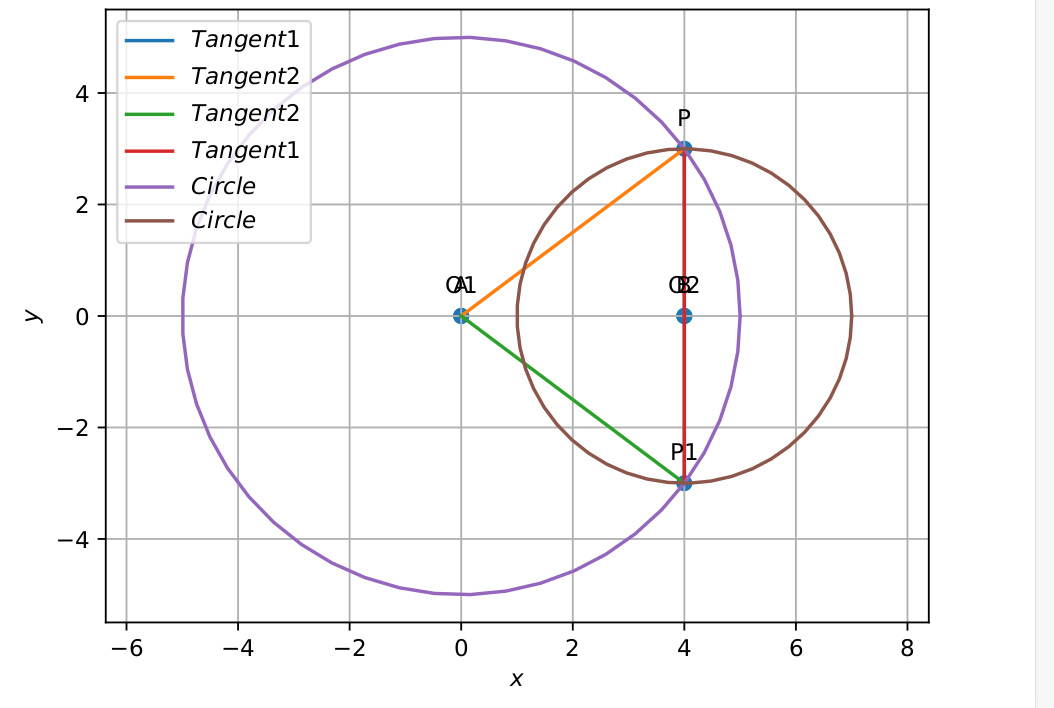
\includegraphics[width=\columnwidth]{cccc.png}
\caption{Diagram generated using python}
\label{fig:square}
\end{figure}
\subsection{Theory:}
{They given two circles radius first circle radii is 5cm(Q1) and  second circle radii is 3cm(Q2) distance between circle 1 and circle 2 is 4cm. we have find the length of the chord.  }

\subsection{Mathematical Calculation:}
$\vec{O} = \myvec{0\\0}$ 
\end{center}
\subsection{Deriving equation for Circle in matrix form}
\vspace{0.2cm}
\begin{flushleft}
The equation of circle in matrix form is,\\
\vspace{0.25cm}
\end{flushleft}
\vspace{0.25cm}
\begin{equation}
 \vec{x}^T \vec{V} \vec{x} + 2 \vec{u}^T \vec{x} + f = 0
\end{equation}
\begin{flushleft}
Where\\
\end{flushleft}
\center
$\vec{V} = \vec{I}= \myvec{ 1 & 0\\ 0 & 1} , \vec{u} = \myvec{0 \\ 0}, \vec{f}=-25$\\
\endcenter
\center
  $\implies$  $ \vec{x}^T$$\vec{I}$ $\vec{x}$  + 2 $ \myvec{0\\0}^T \vec{x} -25 = 0$
\endcenter
\begin{flushleft}
\vspace{0.23cm}
Therefore, the circle equation can be written as
\end{flushleft}
\begin{equation}
    \vec{x}^T \vec{x} + 2 \myvec{0\\0}^T \vec{x} -25= 0
\end{equation}
\endcenter
\begin{flushleft}
The equation of circle in matrix form is,\\
\vspace{0.25cm}
\end{flushleft}
\vspace{0.25cm}
\begin{equation}
 \vec{x}^T \vec{V} \vec{x} + 2 \vec{u}^T \vec{x} + f = 0
\end{equation}
\begin{flushleft}
Where\\
\end{flushleft}
\center
$\vec{V} = \vec{I}= \myvec{ 1 & 0\\ 0 & 1} , \vec{u} = \myvec{-4 \\ 0}, \vec{f}=7$\\
\endcenter
\center
  $\implies$  $ \vec{x}^T$$\vec{I}$ $\vec{x}$  + 2 $ \myvec{-4\\0}^T \vec{x} +7= 0$
\endcenter
\begin{flushleft}
\vspace{0.23cm}
Therefore, the circle equation can be written as
\end{flushleft}
\begin{equation}
    \vec{x}^T \vec{x} + 2 \myvec{-4\\0}^T \vec{x} +7= 0
\end{equation}

\end{equation}
  Here we have to Find the Intersection of Two conics
\begin{equation}
 \vec{x}^T \vec{V_i} \vec{x} + 2 \vec{u_i}^T \vec{x} + f_i = 0
\end{equation}
The locus of their Intersection is a pair of straight lines \\  

\myvec{ \ v_1+\mu v_2 \hspace{10mm} u_1+\mu u_2  \vspace{4mm}\\ u_1+\mu u_2  \hspace{10mm} (f_1+f_2) \\ } \\
\begin{equation}

 \vec{x}^T \vec{(v_1+\mu v_2)}(f1+f2) = (u_1+\mu u_2)(u1+\mu u2)
\end{equation}
\myvec{ 1+\mu \hspace{10mm} 0  \vspace{4mm}\\ 0 \hspace{10mm}  1+\mu \\ } 7\mu \myvec{ 4 , 0} = \myvec{-4\mu , 0} \myvec{-4\mu, 0}\\
\vspace{10mm}
\myvec{7\mu(1+\mu ) \hspace{10mm} 0  \vspace{4mm}\\ 0 \hspace{20mm}  7\mu( 1+\mu) }  =\myvec{16\mu^2\,\hspace{10mm} 0 \vspace{4mm}\\ 0 \hspace{10mm} 0 } \\
\vspace{10mm}
 \mu = -1
 
 \subsection{According to the equation 6}
 2\myvec{-1 \myvec{-4\\0} x }-25-7=0\\
 \vspace{5mm}
 2\myvec{4 , 0 }\myvec{x\\ y} = 32\\
\vspace{5mm}
  8x = 32\\
  \vspace{5mm}
   x=4\\
    \vspace{5mm}
    
    So, p =(4,3)
    \hspace{5mm}
    p_1=(4,-3)
\subsection{ So The length of the common chord is 6cm}
   $$= || p - p_1|| $$
        = \myvec{4\\ 3} - \myvec{4 \\ -3} \\
        \vspace{5mm}
        =6
  \section*{\large Construction}
{
\setlength\extrarowheight{5pt}
\begin{tabular}{|c|c|c|}
  \hline
  \textbf{Symbol}&\textbf{Value}&\textbf{Description}\\
  \hline
	$r_1$&5&Radius \\
  \hline
	$r_2$&3&Radius\\
  \hline
  O&$(0,0)$&Center\\
  \hline
  O_1& $(4,0)$ &Center\\
  \hline
  P&$(4,3)$&Point Of intersection\\
  \hline
  P_1&$(4,-3)$&Point Of intersection\\
  \hline
  P-P_1& $6$ &Length of the common chord\\
  \hline
  
  
\end{tabular}
}
\end{document}